\chapter{New economic and demographic (NED) component}\label{sec:ned-chapter}
The New Economics and Demographics (NED) Module replaces the original Economics and Demographics (ED) module. The initial ED module provided annual predictions of industry activity (output) for the PI module (now replaced with the AA module), employment for the SPG module, and final demand by aggregated industry category for Oregon and scaled those to the full model area using fixed factors. The ED module also reported region-wide construction activity dollars to the ALD module. The demographic portions of the ED module were not used by other modules in the Oregon Statewide Integrated Model. An optional EPF module (no longer used) modified the ED outputs in response to PI model-wide industry location utility trends.

The ED module produced forecasts that were internally consistent, but not necessarily consistent with forecasts from any other model. As a result, a lot of effort went into overriding ED forecasts to develop reference scenarios that were consistent with official state forecasts, which changed every quarter.

The NED module is organized around the concept of scenarios. A scenario is a complete set of NED output that is intended to represent the economic and demographic aspects of a particular future to be modeled. NED outputs are all at the model-region-wide level include forecast output and employment by AA activity, imports and exports by AA commodity, and population by five-year age category. Construction activity and government investment forecasts are reported separately as well. All units are in 2009 dollars, consistent with the rest of SWIM2.

The NED module has three main components:
\begin{enumerate}
\item An exogenously-defined reference scenario that is consistent with assumptions that drive ongoing planning efforts in Oregon.
\item An optional feedback mechanism that allows transportation and land-use policy changes to drive deviations from the way a scenario would progress over time under the policy assumptions that underlie the reference scenario.
\item A scenario generator to allow the definition of alternative economic scenarios to be evaluated
The NED module does not include an economic or demographic model of its own. It consists instead of a representation of the output from exogenous economic and demographic models and the ability to modify those values in appropriate and consistent ways in response to deviations from the reference case in the scenario being evaluated.
\end{enumerate}

A proposed Economic Feedback model (if used) will allow prior year AA modelwide industry location utility trends among other factors to influence NED forecasts, prior to use by other modules. Other NED outputs could also be used to improve consistency and scenario policies, such as SPG to use as constraints the unemployment rate and absolute (rather than distributions of) population by age. 

\section{Theoretical basis}
The change in thinking that led to the replacement of the economics and demographics module (ED) also removed the theoretical basis for having an independent macroeconomic model within SWIM. There remain theoretical bases for the feedback and scenario generation components of NED. 

Feedback modifies current-year NED output in response to deviations from reference-scenario levels in prior year(s) output from other model components. The feedback module operates using elasticities, which define a fixed, linear relationship between proportional change in another module's output and proportional change in a NED quantity. Economic demand and supply functions are almost never linear, but do tend to exhibit fairly constant elasticities, especially over observed ranges of price and quantity. One drawback to relying on elasticities is that when one quantity goes to zero, the other becomes undefined.

If a variable to be fed back is a logsum, it is important that the elasticity to be applied be estimated from logsum data produced using all the same logit-model coefficients that produced the logsum being fed back. Logsum values have no absolute meaning; they have meaning only in relation to other logsums produced from the same logit-model coefficients.

The elasticity parameters to be used in the feedback mechanisms have not yet been estimated. They will be estimated from empirical data and validated against theoretical expectations for their sign and magnitude.

Scenario generation modifies reference-case NED output in future years in advance of running the model based on specifications supplied by the analyst running the model. There is no necessary theoretical basis for the scenarios to be evaluated, but there is a theoretical basis for the translation from the changes in policy variables that the user will have control over and the internal NED variables that the scenario generator will change. The mechanism for translation, which has not yet been implemented, will rely on parameters estimated from empirical data, including input-output model data, and validated against theoretical expectations for their sign and relative magnitude.

\section{Quantity definitions and categories}
NED operates exclusively at the modelwide level. NED produces estimates of employment and output by unsplit AA activity, of imports and exports by commodity\footnote{See the definition of commodities used in the model in Table \ref{tab:goods-categories} on page \pageref{tab:goods-categories}.}, of residential and non-residential construction activity, and of government investment in three categories (federal, state, and capital government accounts). The unsplit AA activity set noted below are further disaggregated by space usage (heavy/light industries and office/non-office) in AA to arrive at the full AA activities noted earlier in Table \ref{tab:activity-industry} (page \pageref{tab:activity-industry}).

\section{Component models}

The NED model involves the following components, described in more detail in the remainder of this section:
\begin{itemize}
\item Reference scenario (exogenously-defined)
\item Feedback mechanism (optional) 
\item Scenario generator (optional)
\end{itemize}
\noindent Each of these are discussed in the following sections.

\subsection{Reference scenario}
The reference scenario is built from external data and forecasts. It starts with IMPLAN data for the model region for 2009 for output, employment, imports, exports, and population. IMPLAN populations are subdivided into five-year age groups using Census data. The 2009 data is kept separate for Oregon and for each of the portions of Washington, Idaho, Nevada, and California that are in the halo. 

\subsubsection{Employment forecasts}
The software implementation of the reference scenario generator allows for separate employment forecasts for each state and a national forecast that substitutes for state forecasts in years for which state forecasts are not available. Oregon provides an official forecast that goes out at least eight years. None of the halo states provide official forecasts more than two years out. Employment growth rates from the Oregon forecast currently are used for all states for the years for which they are available, and then employment growth rates from the national forecast are used. We expect that the actual growth rates in the halo region will more closely resemble Oregon's than the rest of the nation. The national forecast is produced by Global Insight and purchased by the State of Oregon to drive its own forecasting models, including the state forecast we use of Oregon. We therefore expect that the Oregon forecast and the national forecast will be consistent with each other.

Employment is forecast by IMPLAN sector (440 sectors) using a crosswalk that matches one exogenous forecast sector to each IMPLAN sector. Exogenous forecasts have many fewer sectors than IMPLAN and each has its own set of sectors and its own crosswalk. Each year's employment in each IMPLAN sector is forecasted by applying the ratio of that year's employment to the prior year's employment in the corresponding sector in the exogenous forecast to the prior year's employment in that IMPLAN sector.

Employment by state within the model region is aggregated over all states for each IMPLAN sector. Employment by IMPLAN sector is then aggregated to employment by AA activity (52 activities) using a crosswalk that allows IMPLAN sectors to be split among AA activities if necessary. 

\subsubsection{Output forecasts}
For each sector in the national forecast, the ratio of labor productivity (output per employee) in the current year to labor productivity in the prior year is calculated. For each IMPLAN sector in the employment forecast, the minimum of this ratio or 1.05 is applied to the prior years labor productivity within the model region and the resulting, updated labor productivity is multiplied by the forecast of employment for the current year in the model region, yielding forecasted output for that IMPLAN sector in the model region in the current year. 
Output by IMPLAN sector is then aggregated to output by AA activity (52 activities) using a crosswalk that allows IMPLAN sectors to be split among AA activities if necessary. The splits may be different for output than for employment.

\subsubsection{Trade forecasts}
For each IMPLAN sector, the ratio of the current year's output to the base year's output is calculated. Each industry's make of each export commodity from the base-year IMPLAN structural matrices is then scaled by that sector's ratio to get exports by that industry. Each industry's use of each import commodity from the base-year IMPLAN structural matrices is scaled by that sector's ratio to get imports by that industry.

The ratio of current-year population to base-year population is calculated and applied to institutional imports and exports by commodity from the base-year IMPLAN structural matrices to get current year imports and exports by institutions.

Industry and institution imports and exports are aggregated by IMPALN commodity (440 commodities) and then aggregated to AA commodities (52 commodities) using a crosswalk that allows IMPLAN commodities to be split among AA commodities if necessary.

\subsubsection{Construction forecasts}
Construction forecasts are a re-arrangement of the construction output dollars into residential and non-residential structures construction dollars and the exclusion of other non-residential construction activity, such as road building.

\subsubsection{Government forecasts}
Government forecasts use elasticities of government revenue with respect to total employment to estimate state and local government revenue, federal revenues from corporate taxes, and federal revenues from other taxes.

\section{Software implementation}
The NED module and its sub-components are implemented in the Java programming language, and uses Python scripts to execute most NED functions.

\subsection{Reference scenario}
The software implementation of the NED module is a Python script. Each time it is run, it is given a pointer to a parameters file, which it reads to obtain the following parameters:
\begin{itemize}
\item ned.input.directory (where baseline scenario files are read from)
\item ned.activity\_forecast.path (where model-year activity forecast is written)
\item ned.trade\_forecast.path (where model-year trade forecast is written)
\item ned.construction\_forecast.path (where model-year trade forecast is written)
\item ned.population\_forecast.path (where model-year population forecast is written)
\item ned.government\_forecast.path (where model-year government forecast is written)
\item ned.prior\_activity\_forecast.path (where prior-year activity forecast is read from)
\item ned.prior\_trade\_forecast.path (where prior-year trade forecast is read from)
\item ned.prior\_construction\_forecast.path (where prior-year construction forecast is read from)
\item ned.prior\_population\_forecast.path (where prior-year population forecast is read from)
\item ned.prior\_government\_forecast.path (where prior-year government forecast is read from)
\item ned.base.year (e.g., 2009)
\item ned.model.year (an integer value; not a calendar year)
\item ned.base.year.model.year (the model year identifier for the base year)
\item ned.allow.feedback (currently always false)
\end{itemize}

\noindent In the base year, the NED module reads values for that year from the Baseline Scenario files and writes them to that year's NED model files. In subsequent model years, it reads that year's and the prior year's baseline forecast from the Baseline Scenario files, the prior year's model-run forecast, and the prior-year values of feedback variables from other modules.

For each variable in each forecast, the NED module calculates the ratio of this year's value to last year's in the Baseline Scenario. If feedback is enabled, it then adjusts those ratios using the fed-back values from other modules.\footnote{This adjustment is not yet implemented because the variables to be fed back and the elasticities relating change in fed-back variables to changes in NED variables have not yet been identified.} If feedback is not enabled (as is currently always the case), the adjustment factor is 1.0.

The NED module then applies the adjusted ratios to its prior-year forecast to obtain the model-year forecast. The model-year forecasts are then written to the appropriate directories.

Files that NED generates for other modules are written to the appropriate directories as specified in the ned.*\_forecast.path parameters. However, the baseline forecast data that NED uses over time resides in a single directory, specified by the ned.input.directory parameter. The files in that directory are in the same format as the output files except that they have an extra column on the left, in which the year is specified. All NED inputs and outputs represent the entire model region (including Oregon and the halo) and all dollar values are in 2009 dollars.

\subsection{Baseline scenario generator}
The NED Baseline Scenario Generator runs outside of the SWIM2 modeling framework and produces the NED input files that must exist before the SWIM2 model is run. It gathers data from several IMPLAN output files, from state economic forecast files, from the Global Insight national long-run economic forecast files, and from files containing crosswalks and sector mappings. The IMPLAN and forecast files are in their original format, so the Baseline Scenario can be updated by substituting newer copies of the forecast files and then rerunning the Baseline Scenario Generator, without any need to modify the new forecast files. Significant changes in the format of the forecast files by the entity that produces them would require either modifying the code or reformatting the input file. In anticipation of likely changes to forecast files (such as dropping historical years), the code uses named constants to make adjusting the code easy (e.g., a named constant to identify the column in which base-year data are found).

The scenario starts by building internal data structures to hold input values and the results of intermediate calculations. It then reads from various input files and puts their data into the internal data structures. 

Base year results for the Baseline Scenario are calculated by aggregating IMPLAN data to the categories used in SWIM2. IMPLAN population for the model region is attributed to five-year age groups based on 2010 census data proportions. Each subsequent year is then forecasted by applying the appropriate growth rate from each state's forecast to the prior year's employment within that state. If there is no forecast for that state, or if the model year is beyond the end of the state's forecast, the appropriate growth rate from the national forecast is used. Employment is then aggregated over IMPLAN sectors to SWIM2 categories and over states to model region totals.

The states do not forecast output. To forecast output, the ratios of output per employee in each sector in the current year to that in the prior year from the national model is calculated and applied to the prior year's output per employee for the region. The adjusted output per employee is then multiplied by forecasted employment to obtain a forecast of output.

Population in forecasted by applying growth rates by five-year age group from the Oregon population forecast to the prior year's model region population. We do not have population forecasts specific to the halo portions of neighboring states, and assumed that population growth in those counties would be more similar to that in Oregon than to the rest of their states or the nation.

For the trade forecast, industry imports and exports are forecasted separately from institution imports and exports. Industry exports are forecasted by taking the ratio of output for each industry in the model year and the base year and applying it to the exports of each commodity made by that industry in the base year. Industry imports are forecasted by taking the ratio of output for each industry in the model year and the base year and applying it to the imports of each commodity used by that industry in the base year. Imports and exports by institutions (e.g., households and governments) are calculated similarly, but using population ratios rather than output ratios.

The construction forecast used by ALD is constructed by aggregating output dollars from IMPLAN construction sectors.

The government forecast uses estimated elasticities relating change in government revenues to change in employment, which are applied to the change in forecasted employment to get change in government revenue, which is then applied to the prior year's government. The estimated elasticities used are stored in named constants near the top of the script. 

\section{S1 and S2 module parameters}\label{sec:ned-s1-s2}

NED as currently implemented is primarily an exogenous forecast. As such, the Reference Scenario has no estimated parameters, and makes just a few assumptions noted below. In the future the to-be-developed NED Feedback and Scenario Generator model will increase the number of parameters and assumptions. 

The estimated elasticities used in the Reference Scenario government forecast are:
\begin{itemize}
\item FED\_TAX\_ELASTICITY = 1.214
\item SL\_TAX\_ELASTICITY = 1.234
\item CORP\_TAX\_ELASTICITY = 1.054
\end{itemize}

\section{Inputs and Outputs}

The NED input data needed to integrate with the full SWIM2 model components are listed in Table \ref{tab:ned-inputs}. The Reference Scenario as noted was developed from source forecasts, particularly the Oregon OEA forecast and the national Global Insight forecast, along with IMPLAN relationships to disaggregate within Oregon and expand to other states in the halo region of the model. To build this key NED reference scenario input requires the source file datasets listed in Table \ref{tab:ned-source-files}. NED outputs that are used by other parts of SWIM2 are shown in Table \ref{tab:ned-outputs}. NED monetary outputs used by other modules --- AA activity dollars and ALD construction dollars --- are in units of year 2009 dollars, consistent with the rest of the SWIM2 model. 

\begin{table}  % Table 3-1
\centering
\caption{Required inputs for NED}\label{tab:ned-inputs}
\begin{tabular}{L{1.8in} L{3.2in} L{0.85in}}
\hline
Data element & File(s) & Source \\
\hline
Reference scenario forecasts for all years & activity\_forecast.csv, trade\_forecast.csv, government\_forecast.csv, construction\_forecast.csv, population\_forecast.csv & Exogenous \\
\gray Modelwide composite utilities of production activity & ActivitySummary.csv & AA (future) \\
\hline
\end{tabular}
\end{table}

\begin{table}  % Table 3-6 (apparently tables 3-2 through 3-5 never defined)
\centering
\caption{NED source files for the Reference Scenario}\label{tab:ned-source-files}
\begin{tabular}{ll}
\hline
Input file & Data structure \\
\hline
Oregon Industry Detail.xls & implan\_activity \\
\gray Washington Industry Detail.xls & implan\_activity \\
Idaho Industry Detail.xls & implan\_activity \\
\gray Nevada Industry Detail.xls	 & implan\_activity \\
California Industry Detail.xls & implan\_activity \\
\gray OregonAndHalo Industry Detail.xls & implan\_activity \\
cge\_IxI.csv & implan\_structure \\
\gray employment\_annual.xls & state\_forecasts \\
pop\_forecast.xls & population \\
\gray Baseline LR Growth Scenario 2011\_05.xls & national\_forecast \\
implan\_ned\_activity.xls & implan\_ned\_activity \\
\gray implan\_aa\_commodity.xls & implan\_aa\_commodity \\
IMPLAN\_OEA.xls & state\_crosswalks \\
\gray implan\_gi\_sectors.xls & state\_crosswalks \\
\hline
\end{tabular}
\end{table}

\begin{table}
\centering
\caption{NED outputs used by other SWIM2 modules}\label{tab:ned-outputs}
\begin{tabular}{L{3.9in} L{1.6in} L{0.5in}}
\hline
Description & File(s) & Users \\
\hline
Count of modelwide workers by SPG industry & activity\_forecast.csv & SPG1 \\
\gray Modelwide residential and nonresidential final demand of new construction dollars & construction\_forecast.csv & ALD \\
Modelwide quantities of production activity (dollar flows) by AA industry/institution & activity\_forecast.csv, government\_forecast.csv & AA \\
\gray Modelwide quantities of import/export activity (dollar flows) by AA commodity-specific activities & trade\_forecast.csv & AA \\
\hline
\end{tabular}
\end{table}

\section{Validation} 
ED can be compared to the OEA forecast to validate that it is replicating this key source data. Because of the way the reference scenario is built, the rate of employment growth in each sector in the reference scenario is identical to the rate of employment growth in the comparable sector in the OEA employment forecast through the last year of the OEA forecast. 

The following tables show the Reference Scenario quantities and their base-year (2009) values for the model region. This includes employment and output (Table \ref{tab:ned-employment-output}) and population (Table \ref{tab:ned-population-output}) used by SPG. It also includes government accounts (Table \ref{tab:ned-government-accounts}) and trade activity (Table \ref{tab:ned-trade-activity}) used by AA. It also included \$7.89 billion in residential construction and \$7.63 billion in non-residential construction.

\begin{sidewaystable}
\centering
\caption{Model region employment and industry output in the reference scenario base year (2009)}\label{tab:ned-employment-output}
\small
\begin{tabular}{lrr|lrr}
\hline
Activity & Employment & Output & Activity & Employment & Output \\
\hline
CNST\_main\_xxx  & 22,876 & 3,690,346,435 & MFG\_htec\_hi  & 3,634 & 13,063,887,807 \\
\gray CNST\_nRES\_xxx  & 40,908 & 6,542,617,309 & MFG\_htec\_li  & 3,335 & 13,063,887,807 \\
CNST\_offc\_off  & 72,450 & 0 & MFG\_hvtw\_hi  & 22,842 & 14,441,531,006 \\
\gray CNST\_othr\_xxx  & 49,796 & 8,729,001,953 & MFG\_hvtw\_li  & 23,038 & 14,441,531,006 \\
CNST\_RES\_xxx  & 27,477 & 6,740,919,189 & MFG\_lvtw\_hi & 11,756 & 12,978,764,067 \\
\gray ENGY\_elec\_hi  & 5,131 & 8,621,276,855 & MFG\_offc\_off  & 147,103 & 0 \\
ENGY\_ngas\_hi  & 880 & 3,603,145,996 & MFG\_wdppr\_hi  & 25,917 & 11,847,955,596 \\
\gray ENGY\_offc\_off  & 24,548 & 0 & RES\_agmin\_ag  & 98,434 & 16,903,898,303 \\
ENGY\_ptrl\_hi  & 8,672 & 4,631,318,359 & RES\_forst\_log  & 8,356 & 2,519,144,897 \\
\gray ENT\_ENT\_RET & 79,100 & 3,571,715,370 & RES\_offc\_off  & 62,525 & 0 \\
FIRE\_fnin\_off  & 150,334 & 31,902,799,194 & RET\_auto\_RET & 99,235 & 7,439,574,272 \\
\gray FIRE\_real\_off  & 139,465 & 15,446,998,046 & RET\_nstor\_off  & 46,075 & 2,193,797,363 \\
GOV\_admn\_GOV & 101,916 & 19,036,836,853 & RET\_stor\_off  & 56,858 & 0 \\
\gray GOV\_offc\_off  & 162,605 & 0 & RET\_stor\_RET & 229,125 & 16,026,845,092 \\
HIED\_hied\_off\_inst  & 80,247 & 4,569,757,377 & SERV\_bus\_off  & 172,808 & 14,387,504,547 \\
\gray HLTH\_care\_inst  & 68,190 & 3,849,533,203 & SERV\_home\_xxx  & 54,899 & 456,867,797 \\
HLTH\_HOSP\_HOSP & 88,618 & 12,295,007,812 & SERV\_nonp\_off\_inst  & 132,924 & 9,376,816,406 \\
\gray HLTH\_othr\_off\_li  & 150,943 & 18,144,155,090 & SERV\_site\_li & 66,752 & 5,828,886,779 \\
HOSP\_acc\_acc  & 35,825 & 3,539,955,230 & SERV\_stor\_RET & 80,595 & 5,164,732,788 \\
\gray HOSP\_eat\_RET\_acc  & 219,159 & 12,374,280,273 & SERV\_tech\_off  & 219,305 & 22,817,588,607 \\
INFO\_INFO\_off  & 48,211 & 0 & TRNS\_TRNS\_off  & 45,284 & 0 \\
\gray INFO\_INFO\_off\_li  & 9,848 & 15,239,006,202 & TRNS\_TRNS\_ware  & 66,544 & 14,723,200,435 \\
K12\_K12\_K12 & 167,668 & 12,626,084,053 & UTL\_othr\_off  & 14,870 & 0 \\
\gray K12\_K12\_off  & 57,305 & 0 & UTL\_othr\_off\_li  & 17,928 & 8,378,148,941 \\
MFG\_food\_hi  & 14,999 & 10,829,728,776 & WHSL\_offc\_off  & 27,646 & 0 \\
\gray MFG\_food\_li  & 15,124 & 10,829,728,776 & WHSL\_WHSL\_ware & 86,026 & 19,829,592,529 \\
\hline
\end{tabular}
\end{sidewaystable}

\begin{table}
\centering
\caption{Model region population by age in the reference scenario base year (2009)}\label{tab:ned-population-output}
\begin{tabular}{cr|cr}
\hline
Age group & Population & Age group & Population \\
\hline
0 to 4 & 448,259 & 45 to 49 & 451,390 \\
\gray 5 to 9 & 437,565 & 50 to 54 & 457,376 \\
10 to 14 & 449,472 & 55 to 59 & 444,001 \\
\gray 15 to 19 & 465,230 & 60 to 64 & 397,944 \\\
20 to 24 & 463,974 & 65 to 69 & 226,955 \\
\gray 25 to 29 & 456,518 & 70 to 74 & 185,181 \\
30 to 34 & 450,878 & 75 to 79 & 160,906 \\
\gray 35 to 39 & 448,466 & 80 to 84 & 143,361 \\
40 to 44 & 448,611 & 85+ & 120,209 \\
\hline
\end{tabular}
\end{table}

\begin{table}
\centering
\caption{Government accounts for the reference scenario base year (2009)}\label{tab:ned-government-accounts}
\begin{tabular}{lr}
\hline
Government category & Value (2009 \$) \\
\hline
Federal government (FGOV\_acct\_gov) & 93,817,953,918 \\
\gray State and local government (SLGOV\_acct\_gov) & 71,879,103,322 \\
Capitol expenditures (CAP\_acct\_gov) & 69,549,704,567 \\
\hline
\end{tabular}
\end{table}

% Trade activity by commodity monster table (3-10)
\begin{footnotesize}
\begin{longtable}{lr|lr}
\caption{\normalsize{Trade activity by commodity for the reference year base scenario (2009)}}\vspace{-9pt} \\
\hline
Trade activity & Value (2009 \$) & Trade activity & Value (2009 \$) \\ \hline
\endfirsthead
\hline
Trade activity & Value (2009 \$) & Trade activity & Value (2009 \$) \\ \hline
\endhead
\hline \multicolumn{4}{r}{\emph{Continued on next page}}
\endfoot
\hline
\endlastfoot\label{tab:ned-trade-activity}
accommodations\_expt & 3,270,897,187 & sctg17\_pcc\_fuel\_expt & 21,714,405 \\
\gray accommodations\_impt & 2,541,892,752 & sctg17\_pcc\_fuel\_impt & 5,642,668,465 \\
communications and utilities\_expt & 5,678,834,996 & sctg18\_pcc\_petr\_oil\_expt & 10,857,202 \\
\gray communications and utilities\_impt & 7,869,734,616 & sctg18\_pcc\_petr\_oil\_impt & 2,821,334,232 \\
construction\_expt & 9,180,101,387 & sctg19\_pcc\_coal\_prod\_expt & 200,319,354 \\
\gray construction\_impt & 12,590,735,942 & sctg19\_pcc\_coal\_prod\_impt & 4,069,050,714 \\
education reports to sponsors\_expt & 104,924,774 & sctg20\_pcc\_chem\_basic\_expt & 1,126,536,613 \\
\gray education reports to sponsors\_impt & 37,468,124 & sctg20\_pcc\_chem\_basic\_impt & 1,891,511,255 \\
energy\_expt & 3,123,152,392 & sctg21\_pcc\_chem\_pharma\_expt & 764,919,598 \\
\gray energy\_impt & 1,143,833,082 & sctg21\_pcc\_chem\_pharma\_impt & 6,235,158,377 \\
entertainment services\_expt & 407,917,914 & sctg22\_pcc\_chem\_fert\_expt & 179,061,241 \\
\gray entertainment services\_impt & 1,089,285,393 & sctg22\_pcc\_chem\_fert\_impt & 404,925,018 \\
fire business and professional services\_expt & 8,268,890,580 & sctg23\_pcc\_chem\_prod\_expt & 994,754,044 \\
\gray fire business and professional services\_impt & 30,845,752,639 & sctg23\_pcc\_chem\_prod\_impt & 3,300,069,335 \\
food services\_expt & 720,016,802 & sctg24\_pcc\_petr\_plast\_expt & 2,051,431,134 \\
\gray food services\_impt & 333,886,154 & sctg24\_pcc\_petr\_plast\_impt & 4,398,887,943 \\
government administration\_expt & 3,594,244,993 & sctg25\_fwp\_logs\_expt & 1,101,015,179 \\
\gray government administration\_impt & 3,567,099,663 & sctg25\_fwp\_logs\_impt & 340,809,605 \\
health services\_expt & 6,322,315,673 & sctg26\_fwp\_wood\_expt & 4,716,264,380 \\
\gray health services\_impt & 1,230,526,561 & sctg26\_fwp\_wood\_impt & 651,283,882 \\
higher education\_expt & 928,962,118 & sctg27\_ppp\_papr\_puplp\_expt & 4,508,321,602 \\
\gray higher education\_impt & 832,993,534 & sctg27\_ppp\_papr\_puplp\_impt & 840,672,962 \\
personal and other services and amusements\_expt & 4,882,028,098 & sctg28\_ppp\_papr\_paper\_expt & 757,806,729 \\
\gray personal and other services and amusements\_impt & 1,871,340,674 & sctg28\_ppp\_papr\_paper\_impt & 1,240,237,671 \\
retail trade\_expt & 3,929,056,354 & sctg29\_ppp\_papr\_print\_expt & 913,103,214 \\
\gray retail trade\_impt & 1,961,754,163 & sctg29\_ppp\_papr\_print\_impt & 1,703,591,533 \\
sctg01\_fkp\_lvsk\_expt & 402,771,058 & sctg30\_oth\_clth\_expt & 517,835,114 \\
\gray sctg01\_fkp\_lvsk\_impt & 260,851,452 & sctg30\_oth\_clth\_impt & 3,501,242,543 \\
sctg02\_fkp\_agri\_cereal\_expt & 485,384,922 & sctg31\_cms\_min\_expt & 877,088,616 \\
\gray sctg02\_fkp\_agri\_cereal\_impt & 591,333,272 & sctg31\_cms\_min\_impt & 1,356,212,151 \\
sctg03\_fkp\_agri\_other\_expt & 6,652,824,240 & sctg32\_mit\_metl\_base\_expt & 3,018,300,425 \\
\gray sctg03\_fkp\_agri\_other\_impt & 1,099,383,757 & sctg32\_mit\_metl\_base\_impt & 3,520,421,862 \\
sctg04\_fkp\_feed\_expt & 157,695,428 & sctg33\_mit\_metl\_prod\_expt & 2,533,120,109 \\
\gray sctg04\_fkp\_feed\_impt & 763,912,960 & sctg33\_mit\_metl\_prod\_impt & 2,704,359,252 \\
sctg05\_fkp\_food\_meat\_expt & 2,043,552,639 & sctg34\_mit\_mach\_expt & 4,377,044,071 \\
\gray sctg05\_fkp\_food\_meat\_impt & 2,921,116,467 & sctg34\_mit\_mach\_impt & 7,315,651,539 \\
sctg06\_fkp\_agri\_grain\_expt & 761,763,359 & sctg35\_mit\_elct\_expt & 21,885,691,855 \\
\gray sctg06\_fkp\_agri\_grain\_impt & 855,005,202 & sctg35\_mit\_elct\_impt & 11,314,880,451 \\
sctg07\_fkp\_food\_prep\_expt & 9,382,925,853 & sctg36\_mit\_tran\_expt & 3,168,379,696 \\
\gray sctg07\_fkp\_food\_prep\_impt & 5,311,390,317 & sctg36\_mit\_tran\_impt & 6,976,890,863 \\
sctg08\_fkp\_food\_alc\_expt & 1,156,635,454 & sctg37\_mit\_inst\_transp\_expt & 2,603,475,287 \\
\gray sctg08\_fkp\_food\_alc\_impt & 1,431,454,151 & sctg37\_mit\_inst\_transp\_impt & 2,147,223,976 \\
sctg10\_cms\_clay\_expt & 95,534,556 & sctg38\_mit\_inst\_prec\_expt & 2,301,165,169 \\
\gray sctg10\_cms\_clay\_impt & 73,318,169 & sctg38\_mit\_inst\_prec\_impt & 3,143,044,038 \\
sctg11\_cms\_sand\_expt & 163,311,587 & sctg39\_oth\_furn\_expt & 1,103,630,305 \\
\gray sctg11\_cms\_sand\_impt & 17,333,501 & sctg39\_oth\_furn\_impt & 1,872,685,394 \\
sctg13\_cms\_mine\_nonmet\_expt & 34,035,256 & sctg40\_oth\_misc\_expt & 1,856,532,607 \\
\gray sctg13\_cms\_mine\_nonmet\_impt & 144,903,688 & sctg40\_oth\_misc\_impt & 4,774,667,511 \\
sctg14\_cms\_mine\_met\_expt & 1,315,595,424 & sctg41\_waste\_scrap\_expt & 514,256,780 \\
\gray sctg14\_cms\_mine\_met\_impt & 507,173,011 & sctg41\_waste\_scrap\_impt & 470,266,803 \\
sctg15\_pcc\_coal\_expt & 34,023,971 & transport\_expt & 3,152,134,411 \\
\gray sctg15\_pcc\_coal\_impt & 717,887,113 & transport\_impt & 3,101,392,984 \\
sctg16\_pcc\_petr\_crude\_expt & 242,077,538 & wholesale trade\_expt & 3,135,668,823 \\
\gray sctg16\_pcc\_petr\_crude\_impt & 1,590,154,115 & wholesale trade\_impt & 2,033,744,399 \\
\end{longtable}
\end{footnotesize}

The activity levels associated with the Reference Scenario, as of January 2012, covering activity, government, and trade forecasts (used by AA), as well as construction dollar forecasts (used by ALD) are shown in Figures \ref{fig:ned-employment-trends} through \ref{fig:ned-construction-trends}. They are all in terms of percent of 2009 levels, which allows one to compare the growth paths of the different sectors despite some being a lot larger than others.

\begin{figure}
\centering
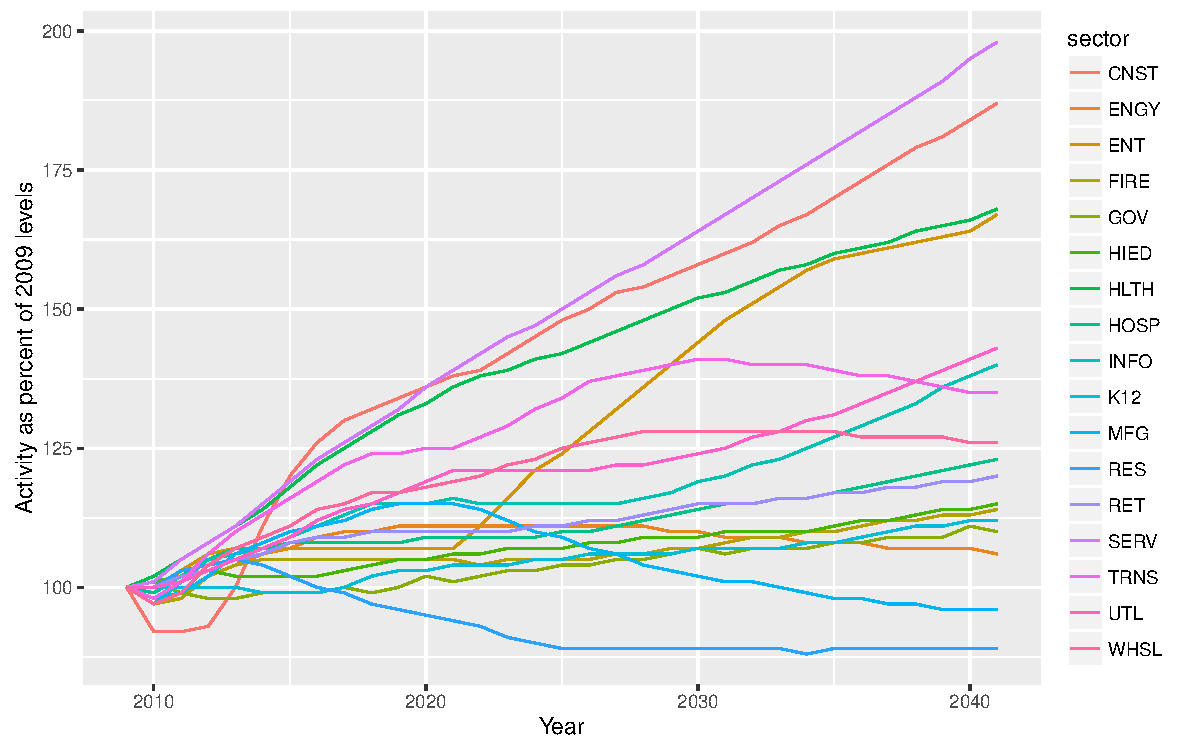
\includegraphics[width=6.5in]{ned/employment_forecast}
\caption{NED reference forecast employment, 2009-40}\label{fig:ned-employment-trends}
\end{figure}

\begin{figure}
\centering
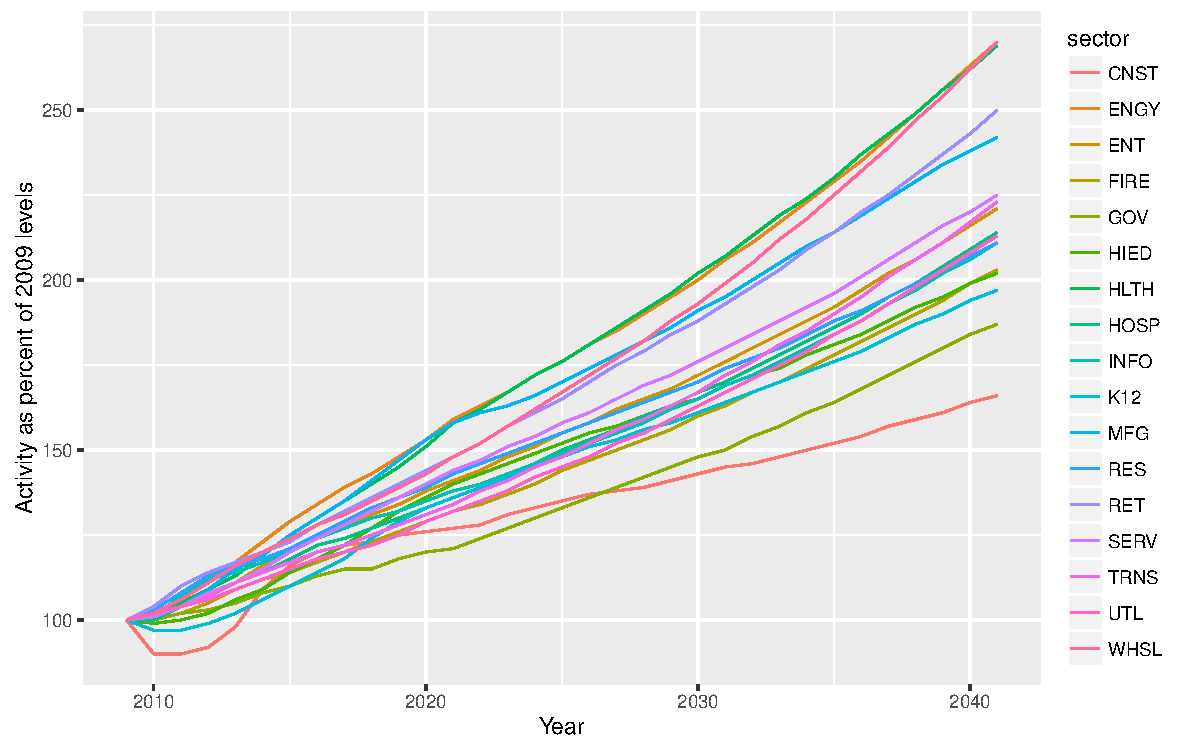
\includegraphics[width=6.5in]{ned/activity_forecast}
\caption{NED reference forecast industry activity, 2009-40}
\end{figure}

\begin{figure}
\centering
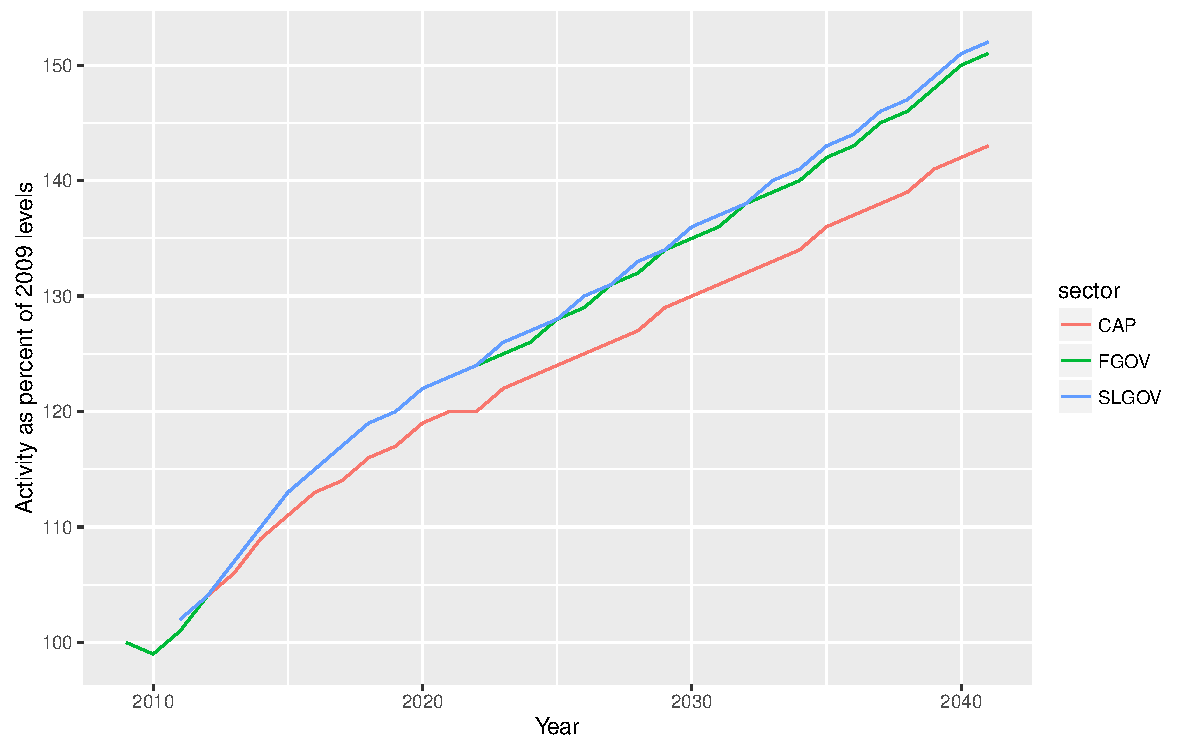
\includegraphics[width=6.5in]{ned/government_forecast.pdf}
\caption{NED reference forecast government activity, 2009-40}
\end{figure}

\begin{figure}
\centering
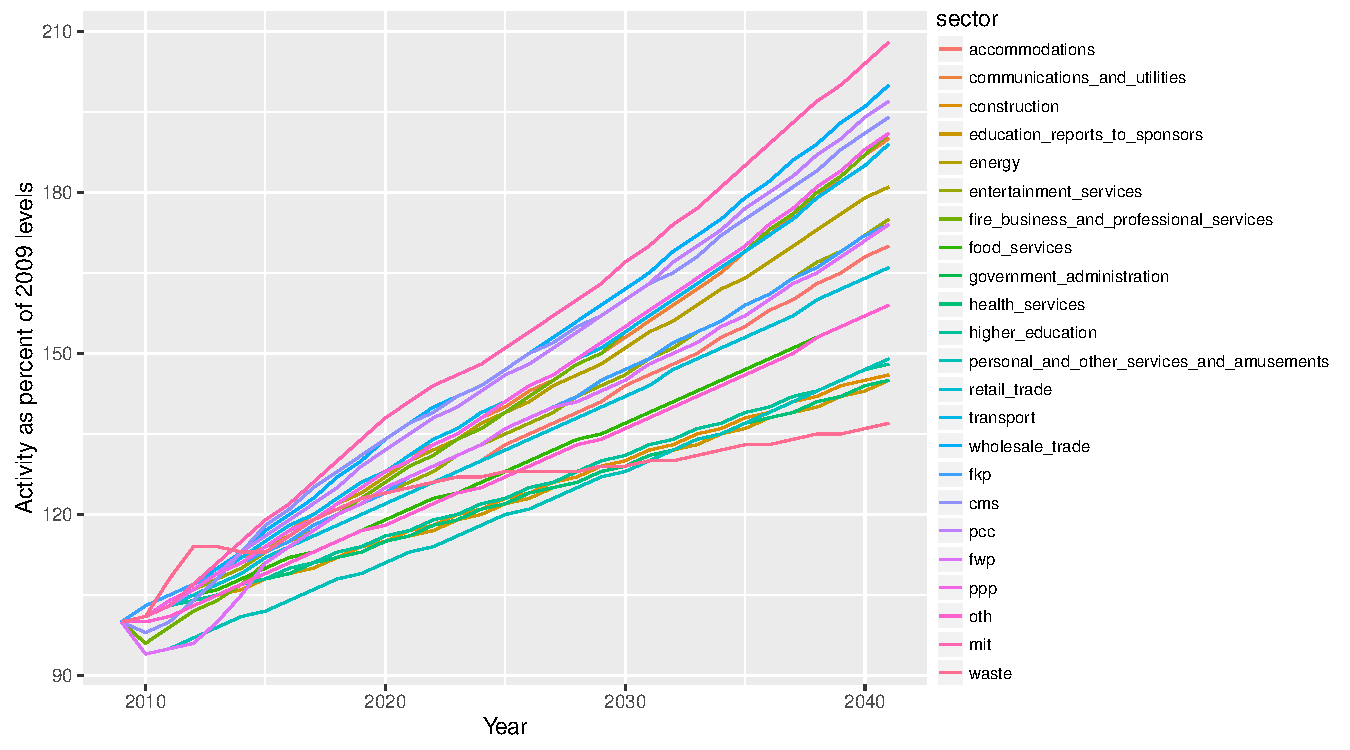
\includegraphics[width=7in]{ned/trade_forecast_imports.pdf}
\caption{NED reference forecast import activity, 2009-40}
\end{figure}

\begin{figure}
\centering
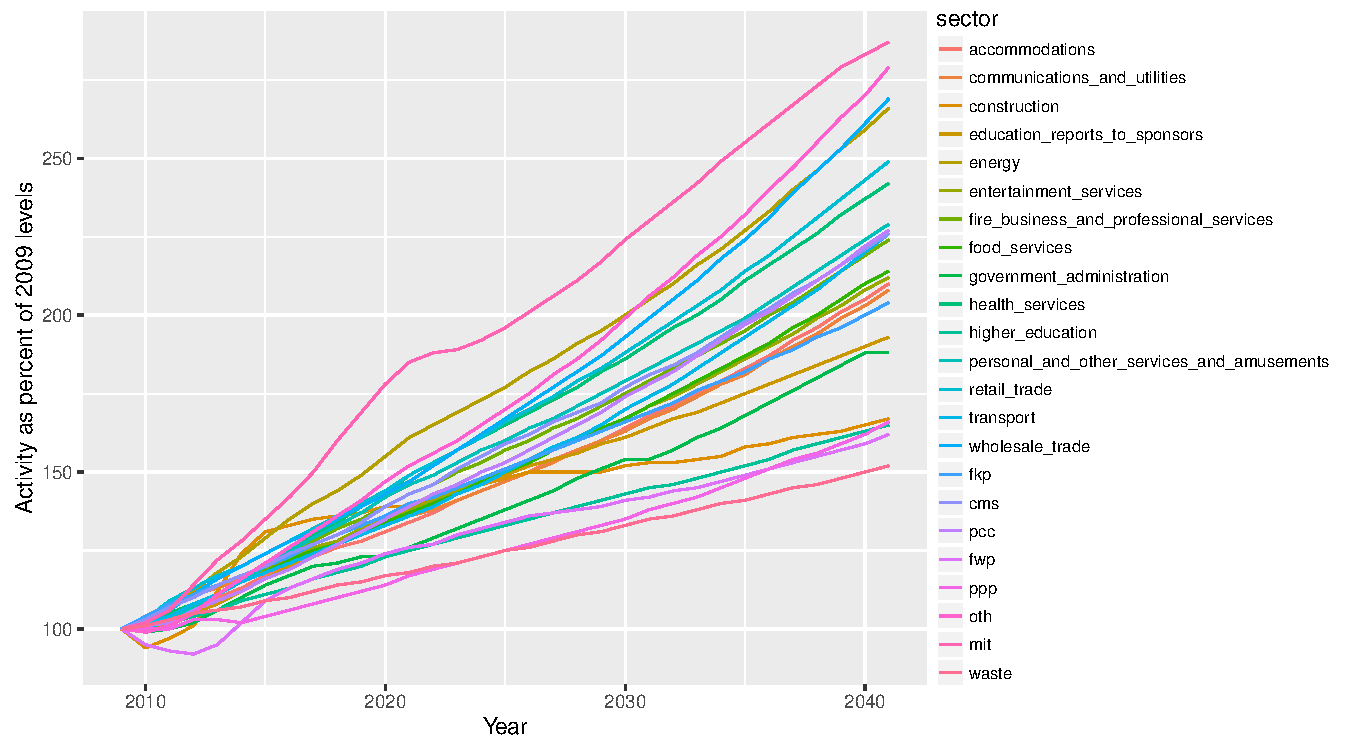
\includegraphics[width=7in]{ned/trade_forecast_exports}
\caption{NED reference forecast export activity, 2009-40}
\end{figure}

\begin{figure}
\centering
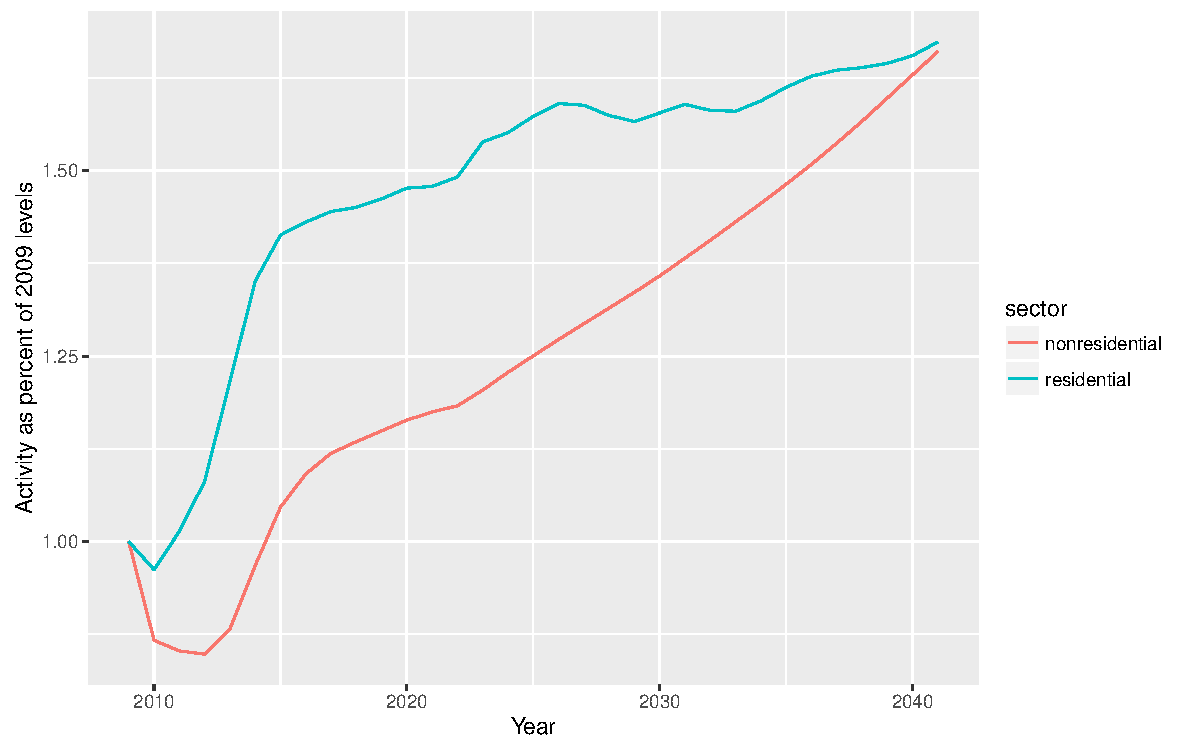
\includegraphics[width=6.5in]{ned/construction_forecast}
\caption{NED reference forecast annual construction dollars, 2009-40}
\label{fig:ned-construction-trends}
\end{figure}

\section{S3 Parameters}
The few estimated ED module coefficients, as well as the structure of the ED module (the number and composition of the equations) may be considered S3 parameters, subject to re-estimation and refinement as the full SWIM Model is tested and calibrated.

\section{Future Plans}
In the near future, the feedback features in NED will be made operational, parameterized, calibrated, and validated. A scenario generation tool also will be developed, allowing the model user to specify alternative scenarios. The scenario generation tool will produce files identical in format to those produced by the Baseline Scenario Generator, as well as files specifying alternative data for other modules. When an alternative scenario is run, those variables that differ from their counterparts in the baseline scenario will not be subject to change via feedback; the specification of the alternative scenario will be maintained. Other variables that are not a part of the specification may respond to feedback if feedback is enabled.

